%!Mode:: "TeX:UTF-8"
\documentclass[a4paper,11pt,UTF8]{ctexart}

\usepackage{indentfirst} %缩进
\usepackage{xeCJK}    %使用系统字体
\usepackage{fancyhdr} %自定义页眉页脚
\pagestyle{empty}                   %不设置页眉页脚
\usepackage{amsmath, amsthm, amssymb, amsfonts} %数学公式
\usepackage[a4paper,left=3cm,right=3cm,top=3cm,bottom=3cm]{geometry}
%\usepackage[tmargin=1in,bmargin=1in,lmargin=1.25in,rmargin=1.25in]{geometry}.
\usepackage{booktabs} %插入表格
\usepackage[section]{placeins} %避免浮动
\usepackage{listings} %插入代码
\usepackage{ctex}     %中文宏包
\usepackage[svgnames, table]{xcolor} %彩色表格
\usepackage{algorithm}          %伪代码
\usepackage{algorithmicx}
\usepackage{algpseudocode}
\usepackage{algorithm,algpseudocode,float}
\usepackage{lipsum}
\usepackage{enumitem}           %调整列举环境
\usepackage{url}
\usepackage{fontspec,xunicode}
\defaultfontfeatures{Mapping=tex-text} %如果没有它,会有一些 tex 特殊字符无法正常使用,比如连字符。

\usepackage{graphicx}
\graphicspath{{imgs/}}
\usepackage{physics}
%%%%%%%%%%%%%%%%%%%%%%%%%%%%%%%%%%%%%%%%%%%%%%%%%%%%%%%%%%%%%%%%
% 缩进及行间距
%%%%%%%%%%%%%%%%%%%%%%%%%%%%%%%%%%%%%%%%%%%%%%%%%%%%%%%%%%%%%%%%
\setlength{\parindent}{0pt} %重新定义缩进长度
\setlength{\baselineskip}{20pt}  %定义行间距
%\renewcommand{\baselinestretch}{1.1} %定义行间距

%%%%%%%%%%%%%%%%%%%%%%%%%%%%%%%%%%%%%%%%%%%%%%%%%%%%%%%%%%%%%%%%
% 列表设置
%%%%%%%%%%%%%%%%%%%%%%%%%%%%%%%%%%%%%%%%%%%%%%%%%%%%%%%%%%%%%%%%
\setenumerate{fullwidth,itemindent=\parindent,listparindent=\parindent,itemsep=0ex,partopsep=0pt,parsep=0ex}
\setenumerate[2]{label=\alph*),leftmargin=1.5em}  %二级item设置
\setitemize{itemindent=38pt,leftmargin=0pt,itemsep=-0.4ex,listparindent=26pt,partopsep=0pt,parsep=0.5ex,topsep=-0.25ex}
\setdescription{itemindent=38pt,leftmargin=0pt,itemsep=-0.4ex,listparindent=26pt,partopsep=0pt,parsep=0.5ex,topsep=-0.25ex}

%%%%%%%%%%%%%%%%%%%%%%%%%%%%%%%%%%%%%%%%%%%%%%%%%%%%%%%%%%%%%%%%
% 图的标题行间距设置
%%%%%%%%%%%%%%%%%%%%%%%%%%%%%%%%%%%%%%%%%%%%%%%%%%%%%%%%%%%%%%%%
\newcommand{\bottomcaption}{%
\setlength{\abovecaptionskip}{6pt}%
\setlength{\belowcaptionskip}{6pt}%
\caption}


%%%%%%%%%%%%%%%%%%%%%%%%%%%%%%%%%%%%%%%%%%%%%%%%%%%%%%%%%%%%%%%%
% 字体定义
%%%%%%%%%%%%%%%%%%%%%%%%%%%%%%%%%%%%%%%%%%%%%%%%%%%%%%%%%%%%%%%%
\setmainfont{Times New Roman}  %默认英文字体.serif是有衬线字体sans serif无衬线字体
\setmonofont{Consolas}
\setCJKmainfont[ItalicFont={楷体}, BoldFont={黑体}]{宋体}%衬线字体 缺省中文字体为
\setCJKsansfont{黑体}
\punctstyle{hangmobanjiao}
%-----------------------xeCJK下设置中文字体------------------------------%
\setCJKfamilyfont{song}{SimSun}                             %宋体 song
\newcommand{\song}{\CJKfamily{song}}
\setCJKfamilyfont{fs}{FangSong}                      %仿宋  fs
\newcommand{\fs}{\CJKfamily{fs}}
\setCJKfamilyfont{ktgb}{KaiTi}                      %楷体2312 ktgb
\newcommand{\ktgb}{\CJKfamily{ktgb}}
\setCJKfamilyfont{yh}{Microsoft YaHei}                    %微软雅黑 yh
\newcommand{\yh}{\CJKfamily{yh}}
\setCJKfamilyfont{hei}{SimHei}                              %黑体  hei
\newcommand{\hei}{\CJKfamily{hei}}
\setCJKfamilyfont{hwxk}{STXingkai}                                %华文行楷  hwxk
\newcommand{\hwxk}{\CJKfamily{hwxk}}
%------------------------------设置字体大小------------------------%
\newcommand{\shiyanbaogao}{\fontsize{36pt}{\baselineskip}\selectfont}
\newcommand{\chuhao}{\fontsize{42pt}{\baselineskip}\selectfont}     %初号
\newcommand{\xiaochuhao}{\fontsize{36pt}{\baselineskip}\selectfont} %小初号
\newcommand{\yihao}{\fontsize{28pt}{\baselineskip}\selectfont}      %一号
\newcommand{\erhao}{\fontsize{21pt}{\baselineskip}\selectfont}      %二号
\newcommand{\xiaoerhao}{\fontsize{18pt}{\baselineskip}\selectfont}  %小二号
\newcommand{\sanhao}{\fontsize{15.75pt}{\baselineskip}\selectfont}  %三号
\newcommand{\sihao}{\fontsize{14pt}{\baselineskip}\selectfont}       %四号
\newcommand{\xiaosihao}{\fontsize{12pt}{\baselineskip}\selectfont}  %小四号
\newcommand{\wuhao}{\fontsize{10.5pt}{\baselineskip}\selectfont}    %五号
\newcommand{\xiaowuhao}{\fontsize{9pt}{\baselineskip}\selectfont}   %小五号
\newcommand{\liuhao}{\fontsize{7.875pt}{\baselineskip}\selectfont}  %六号
\newcommand{\qihao}{\fontsize{5.25pt}{\baselineskip}\selectfont}    %七号

%%%%%%%%%%%%%%%%%%%%%%%%%%%%%%%%%%%%%%%%%%%%%%%%%%%%%%%%%%%%%%%%
% 图题字体大小相同
%%%%%%%%%%%%%%%%%%%%%%%%%%%%%%%%%%%%%%%%%%%%%%%%%%%%%%%%%%%%%%%%
\usepackage{caption}
\captionsetup{font={footnotesize}}   % footnotesize = 9pt
\captionsetup[lstlisting]{font={footnotesize}}

%%%%%%%%%%%%%%%%%%%%%%%%%%%%%%%%%%%%%%%%%%%%%%%%%%%%%%%%%%%%%%%%
% 重定义枚举编号为 1),2)...
%%%%%%%%%%%%%%%%%%%%%%%%%%%%%%%%%%%%%%%%%%%%%%%%%%%%%%%%%%%%%%%%
\renewcommand{\labelenumi}{\theenumi)}

%%%%%%%%%%%%%%%%%%%%%%%%%%%%%%%%%%%%%%%%%%%%%%%%%%%%%%%%%%%%%%%%
% 标题名称中文化
%%%%%%%%%%%%%%%%%%%%%%%%%%%%%%%%%%%%%%%%%%%%%%%%%%%%%%%%%%%%%%%%
\renewcommand\figurename{\hei 图}
\renewcommand\tablename{\hei 表}
\renewcommand\lstlistingname{\hei 代码}
\renewcommand{\algorithmicrequire}{\textbf{输入:}}
\renewcommand{\algorithmicensure}{\textbf{输出:}}
\newtheorem{define}{定义}

%%%%%%%%%%%%%%%%%%%%%%%%%%%%%%%%%%%%%%%%%%%%%%%%%%%%%%%%%%%%%%%%
% 代码设置
%%%%%%%%%%%%%%%%%%%%%%%%%%%%%%%%%%%%%%%%%%%%%%%%%%%%%%%%%%%%%%%%
\lstset{
 columns=fixed,
 numbers=left,                                        % 在左侧显示行号
 numberstyle=\tiny\color{gray},                       % 设定行号格式
 frame=single,                                        % 单线背景边框
 breaklines=true,                                     % 设定LaTeX对过长的代码行进行自动换行
 keywordstyle=\color[RGB]{40,40,255},                 % 设定关键字颜色
 numberstyle=\footnotesize\color{darkgray},
 commentstyle=\it\color[RGB]{0,96,96},                % 设置代码注释的格式
 stringstyle=\rmfamily\slshape\color[RGB]{128,0,0},   % 设置字符串格式
 showstringspaces=false,                              % 不显示字符串中的空格
 language=java,                                        % 设置语言
 basicstyle=\linespread{1.0}\xiaowuhao\ttfamily,                      % 字体字号
 %lineskip=10pt,
 %baselinestretch=1,
}

%%%%%%%%%%%%%%%%%%%%%%%%%%%%%%%%%%%%%%%%%%%%%%%%%%%%%%%%%%%%%%%%
% 伪代码分页
%%%%%%%%%%%%%%%%%%%%%%%%%%%%%%%%%%%%%%%%%%%%%%%%%%%%%%%%%%%%%%%%
\makeatletter
\renewcommand{\ALG@name}{算法}
\newenvironment{breakablealgorithm}
  {% \begin{breakablealgorithm}
   \begin{center}
     \refstepcounter{algorithm}% New algorithm
     \hrule height.8pt depth0pt \kern2pt% \@fs@pre for \@fs@ruled
     \renewcommand{\caption}[2][\relax]{% Make a new \caption
       {\raggedright\textbf{\ALG@name~\thealgorithm} ##2\par}%
       \ifx\relax##1\relax % #1 is \relax
         \addcontentsline{loa}{algorithm}{\protect\numberline{\thealgorithm}##2}%
       \else % #1 is not \relax
         \addcontentsline{loa}{algorithm}{\protect\numberline{\thealgorithm}##1}%
       \fi
       \kern2pt\hrule\kern2pt
     }
  }{% \end{breakablealgorithm}
     \kern2pt\hrule\relax% \@fs@post for \@fs@ruled
   \end{center}
  }
\makeatother

% =============================================
% Part 1 Edit the info
% =============================================



\newcommand{\course}{电子线路实验(1)}
\newcommand{\newtitle}{加法器及其应用}
\title{加法器及其应用}
\author{PB19000132苗立扬  PB18020556 戴佳乐}

% =============================================
% Part 1 Main document
% =============================================
\begin{document}
\maketitle

% =============================================
% Part 2 Main document
% =============================================

%
\newcommand{\p}{\par}
\newcommand{\np}{\par\noindent}
%
\newcommand{\expa}{用一片74LS283实现并行四位全加,将A置为1001,B置为0000\~{}1001,
依次计算A+B并记录结果表列。}
\newcommand{\expb}{用两片74LS283和必要的门电路实现两个8421BCD码求和运算,结果
仍为8421BCD码,要求画出逻辑功能图。}
\newcommand{\expc}{用两片74LS283和必要的门电路实现一个带借位输入和借位输出的
8421BCD码减法器,要求电路输出为原码}
\newcommand{\expd}{用双4选1数据选择器74LS153实现一位全加器}
\newcommand{\chip}{数据选择器74LS151}

\newcommand{\CI}{C\negthinspace I}
\newcommand{\CO}{C\negthinspace O}
%

\section{实验目的}

(1)掌握组合逻辑电路的设计方法,理解半加器和全加器的逻辑功能。\\
(2)掌握中规模集成电路加法器的工作原理及其逻辑功能。\\


\section{实验原理}

在数字系统中,经常需要进行算术运算,逻辑操作及数字大小比较等操作,实现这些运算功能的电路是加法器。
加法器是一种组合逻辑电路,主要功能是实现二进制数的算术加法运算。
\\

 \subsection{半加器}
 (1)半加器完成两个一位二进制数相加,若只考虑两个加数本身,而不考虑来自相邻低位的进位,
 称为半加,实现半加运算功能的电路称为半加器。\\
 \begin{figure}[H]
  \centering
  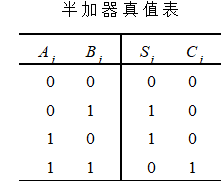
\includegraphics[width=6cm]{jfqpic1}
  \caption{半加器真值表}
  \label{fig:jfqpic1}
\end{figure}
 (2)由真值表可得出半加器的逻辑表达式,见图1。\\
 (3)其逻辑表达式、逻辑图及符号见图2。
 \begin{figure}[H]
  \centering
  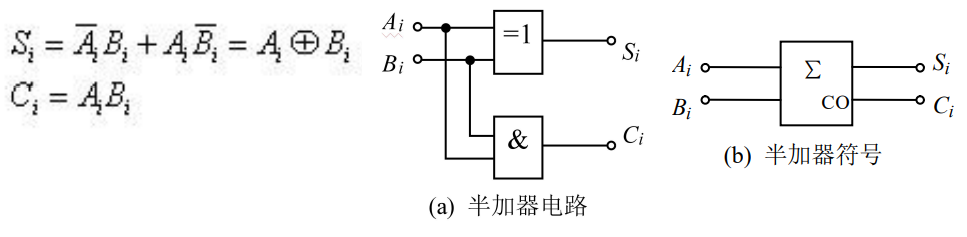
\includegraphics[width=14cm]{jfqpic2}
  \caption{半加器逻辑表达式、逻辑图及符号}
  \label{fig:jfqpic2}
 \end{figure}
 \subsection{全加器}
 (1)两个多位数相加是每一位都是带进位相加,所以必须用全加器。这时只要依
 次将低位的进位输出接到高位的输入,就可构成多位加法器了。\\
 (2)全加器是一种由被加数、加数和来自低位的进位数三者相加的运算器。基本
 功能是实现二进制加法。\\
 (3)逻辑表达式:
 \begin{figure}[H]
  \centering
  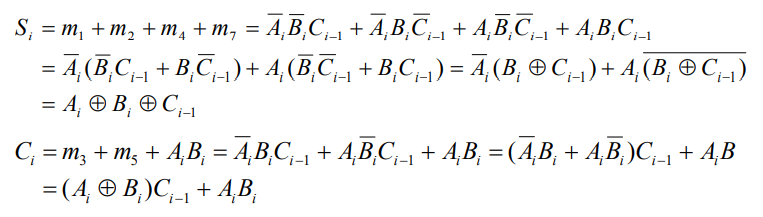
\includegraphics[width=12cm]{jfqpic3}
  \caption{全加器逻辑表达式}
  \label{fig:jfqpic3}
 \end{figure}
 (4)全加器真值表、逻辑图及符号:
 \begin{figure}[H]
  \centering
  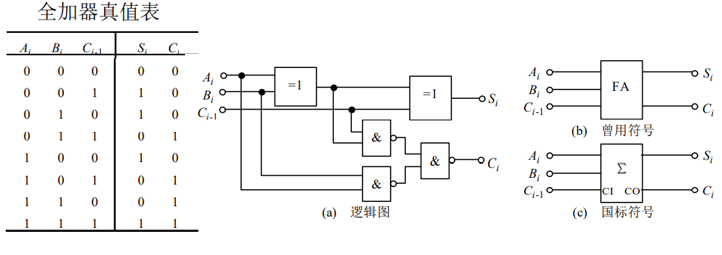
\includegraphics[width=12cm]{jfqpic4}
  \caption{全加器真值表、逻辑图及符号}
  \label{fig:jfqpic4}
 \end{figure}
 \subsection{串行进位加法器}
 \begin{figure}[H]
  \centering
  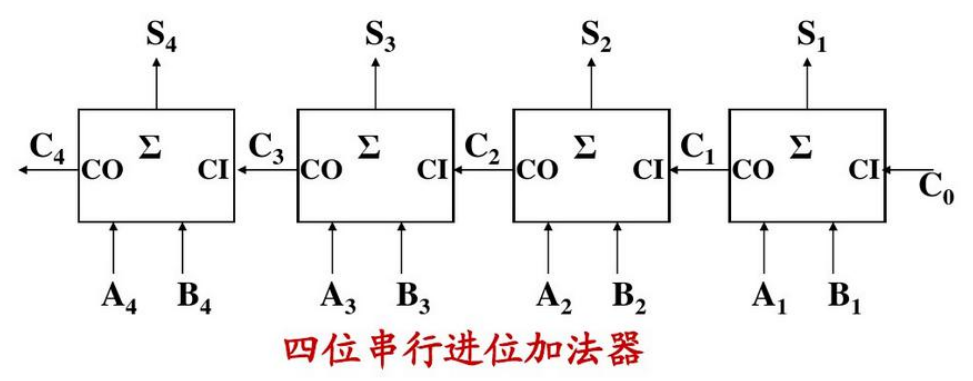
\includegraphics[width=14cm]{jfqpic5}
  \caption{四位串行进位加法器}
  \label{fig:jfqpic5}
 \end{figure}
 特点:结构简单、运算速度慢。
 \subsection{并行加法器}
  \subsubsection{进位链}
  把n个加法器单元电路按一定方式互联起来,即构成n位的并行加法器。其由两部分组成:
  (1)并行成分,指两个操作数的所有位同时并行加入加法器运算;\\
  (2)链结构。\\
  虽然操作数各位同时加入加法器进行运算,但并非所有位和数都同时产生,
  它存在进位的产生与传送问题,进位的产生与传送称为进位链,
  它的结构是影响加法器速度的关键。
  \subsubsection{先行进位}
  先行进位也称并行进位,指加法器各位的进位是各自独立且同时产生的,
  高一位的进位不依赖低位的进位产生与传送。
  并行加法器任何一位的进位:
  \begin{equation}
    C_i=A_iB_i+(A_i\oplus B_i)C_{i-1}=A_iB_i+(A_i+B_i)C_{i-1}
  \end{equation}
  它可以分为两个部分,$A_iB_i$和$(A_i\oplus B_i)C_{i-1}$,前者仅与这一位的两个操作数有关,与低位的进位无关,
  称它为本地进位或进位生成函数,记为$G_i$;后者不仅与操作数有关,还与低位的进位有关,
  称它为传递进位,称$(A_i\oplus B_i)$或$(A_i+B_i)$为传递函数$P_i$。因此可以写成:
  \begin{equation}
    C_i=G_i+P_iC_{i-1}
  \end{equation}
 \subsection{超前进位并行加法器}
 (1)超前进位电路构成的快速进位的4位全加器电路74LS283,可实现两个四位二进制的全加。
 \begin{figure}[H]
  \centering
  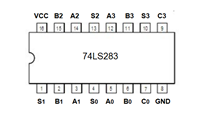
\includegraphics[width=8cm]{jfqpic7}
  \caption{74LS283集成芯片引脚图}
  \label{fig:jfqpic7}
 \end{figure}
 (2)加进位输入$C_0$和进位输出$C_3$主要用来扩大加法器字长,作为组间行波进位之用。
 由于它采用超前进位方式,所以进位传送速度快。
 \begin{figure}[H]
  \centering
  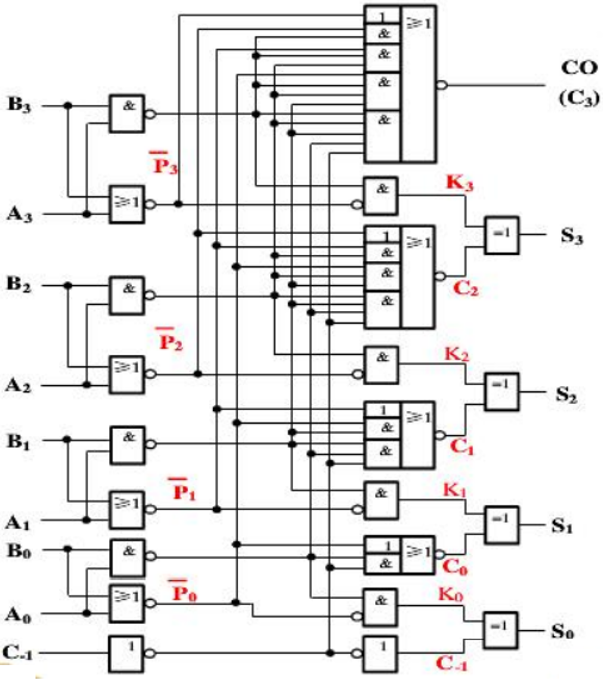
\includegraphics[width=10cm]{jfqpic8}
  \caption{74LS283电路图}
  \label{fig:jfqpic8}
 \end{figure}



\section{实验内容、步骤与结果}
 \subsection{实验一:\expa}
 \begin{figure}[H]
  \centering
  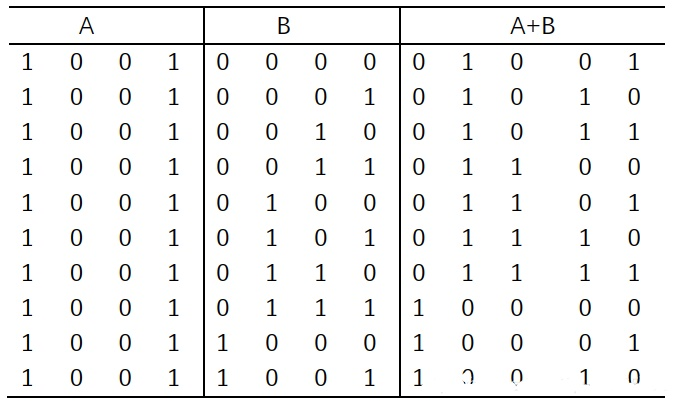
\includegraphics[width=12cm]{jfqpic9}
  \caption{A+B记录表}
  \label{fig:jfqpic9}
 \end{figure}












 
 \subsection{实验二:\expb}
 \begin{figure}[H]
  \centering
  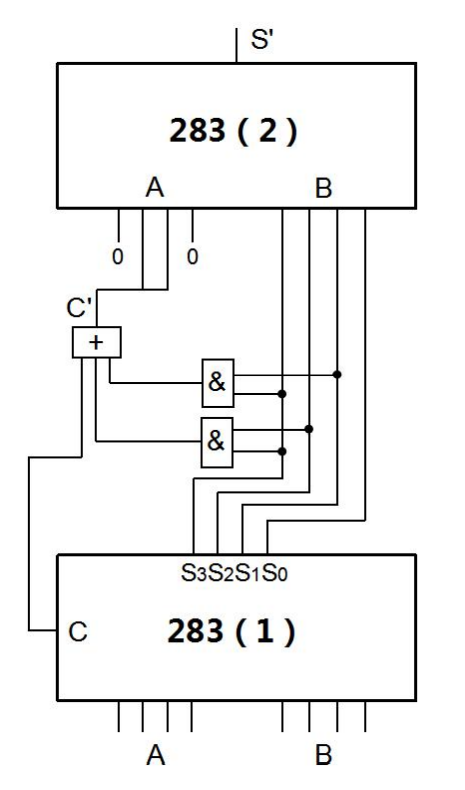
\includegraphics[width=8cm]{jfqpic10}
  \caption{8421BCD码加法器电路}
  \label{fig:jfqpic10}
 \end{figure}
 
% Table generated by Excel2LaTeX from sheet 'Sheet1'
\begin{table}[htbp]
	\centering
	
	\begin{tabular}{|c|c|c|}
		\hline
		A     & B     & 显示 \\\hline
		0111  & 0101  & 12 \\\hline
		0100  & 0100  & 8 \\\hline
		1010  & 0001  & 11 \\\hline
		1011  & 0010  & 13 \\\hline
	\end{tabular}%
	\caption{8421CD码求和结果表}
	\label{tab:addlabel}%
\end{table}%




  


  
 

\section{总结}
通过这次实验,本组同学掌握了组合逻辑电路的设计方法,理解了半加器和全加器的逻辑功能,
掌握了中规模集成电路加法器的工作原理及其逻辑功能。
\\
使用门电路实现半加器与全加器时,首先应列出半加器真值表或全加器真值表,
然后由真值表得到逻辑表达式,再通过化简,画出逻辑电路图。\\
使用四位二进制全加器74LS283设计代码转换电路时,由于具有加法器功能,所以很方便进行转换。
比如8421转换为余3码,余3码与8421码相差3,所以加三就可以得到余3码。
相差部分,只需要用283进行加法。

 




\section{思考题}
 \subsection{\expc}

 283原本是四位全加器,这里用于做减法器,很自然想到用补码代替被减数做加法运算。\\
 $A$四位输入,$B$四位输入。做$A-B$。$C_i$为借位输入,即低位向$A$借位,由于是二进制运算,
 所以借位只会为0或1。$C_0$为借位输出,即$A-B$向高位借位,也为0或1。283本身有一个进位输入,
 将其取反引出作为$C_i$输入。无借位输入时,$B$反码加1,有借位输入时$B$反码不加。$B$取
 反码输入,连接283前先通过反相器。第一片283进位输出取反为$C_0$。若$A<B$,$C_0$
 为1,此时第一片输出结果为补码,需要用第二片283取补码。逻辑电路图如下:
 \begin{figure}[H]
  \centering
  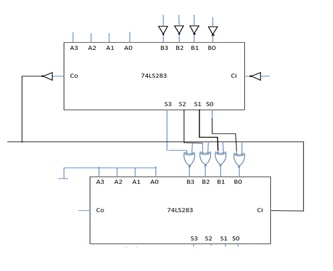
\includegraphics[width=10cm]{jfqpic13}
  \caption{8421BCD码减法器电路图}
  \label{fig:jfqpic13}
 \end{figure}
 \newpage
 第一片283输出,与$C_0$做异或,因为若没有进位输出,说明减法结果为正数,不需要求补码。
 若结果为负数,此时$C_0$为1,则第一片283输出取反输入第二片283,同时$C_0$作为第二片$C_i$,
 因为取反加一为补码,第二片输出结果为$A-B$的差值绝对值。







\end{document}
